\documentclass{article}
\usepackage[cm,plain]{fullpage}
\usepackage{enumerate}           % This package gives fancier enumeration styles
\usepackage{times}               % This package provides use of Times font
\usepackage{graphicx}            % This package provides use of graphics


%==============================================================
% EDIT: Change your name and the assignment number if necessary.
\author{John Devivo}          % Use your name instead
\title{Homework \#2}       % Note the \ before the # symbol 
                           % # is a special character

%==============================================================
% This is where the real document begins
% 1.(12,17,19,36,38,43)

\begin{document}
\maketitle
\begin{center}     % Start a centered block of text
\Large{\bf Due: Tuesday, September 16}\\
Collaborators: Ryan Schwarz
\end{center}       % Centering ends here

\section*{E-1.12}

Let $D = \{ w | w$ contains an even number of a's and an odd number of b's
and does not contain the substring {\tt ab}$\}$.
Give a DFA with five states that recognizes $D$ and a regular expression
that generates $D$. (Suggestion: Describe $D$ more simply.)

{\bf Answer: } The DFA should be saved as the file \verb=1_12.jff=.
The regular expression is  $b(bb)^*(aa)^*$

\section*{E-1.17}
% a,b

\begin{enumerate}[a.]
\item Give an NFA recognizing the language $(01 \cup 001 \cup 010)^*$.\\
{\bf Answer: } The NFA should be saved as the file \verb=1_17_a.jff=.
\item Convert this NFA to an equivalent DFA.
Give only the portion of the DFA that is reachable from the start state.\\
{\bf Answer: } The DFA should be saved as the file \verb=1_17_b.jff=.
\end{enumerate}

\section*{E-1.19}
% a,b

Use the procedure described in Lemma 1.55 to convert the following regular
expressions to nondeterministic finite automata.
\begin{enumerate}[a.]
\item $(0 \cup 1)^*000(0 \cup 1)^*$\\
{\bf Answer: } The NFA should be saved as the file \verb=1_19_a.jff=.
\item $(((00)^*(11)) \cup 01)^*$\\
{\bf Answer: } The NFA should be saved as the file \verb=1_19_b.jff=.
\end{enumerate}

\section*{E-1.36}

Let $B_n = \{a^k | k \mbox{\ is a multiple of $n$}\}$.  Show
that for each $n \geq 1$, the language $B_n$ is regular.

{\bf Answer: } 
For every multiple of $n$, $k$, where $n \geq 1$, $k$ is an integer where $k \geq 1$. We also know that every $a$, raised to a positive integer is a regular language.  Knowing this we can say that all $a^k$ are regular languages. We also know that the union of any number of regular languages will represent a regular language. $B_n$ is the union of all $a^k$ and each $a^k$ represents a regular language. Knowing this we can say that $B_n$ is a regular language.

\section*{E-1.38}

An \emph{all}-NFA $M$ is a 5-tuple $(Q, \Sigma, \delta, q_0, F)$ that
accepts $x \in \Sigma^*$ if {\em every} possible state that $M$ coud be in 
after reading input $x$ is a state from $F$.
Note, in contrast, that an ordinary NFA accepts a string if some state among
these possible states is an accept state.
Prove that all-NFAs recognize the class of regular languages.

{\bf Answer: } In an all-NFA, the set of accept states $F$ can be described as $F=\Sigma^*$, where $\Sigma$ is the alphabet. We can prove that an all-NFA represents a regular language in two ways, proving it can be converted to a regular expression, or proving that all all-NFAs can be converted to regular NFAs. Showing that an all-NFA can be converted to a regular expression is easiest. Using the same alphabet, every all-NFA can be represented as the regular expression $\Sigma^*$ since the set of accept string for and all-NFA is the set $\Sigma^*$. Since we can convert every all-NFA of any alphabet to an equivalent regular expression, all-NFAs are regular. 

\section*{E-1.43}

Let $A$ be any language.
Define DROP-OUT(A) to be the language containing all strings that can be obtained by removing
one symbol from a string in $A$.
Thus, DROP-OUT(A) = $\{xz | xyz \in A \mbox{\ where $x,z \in \Sigma^*, y \in \Sigma$}\}$.
Show that the class of regular languages is closed under the DROP-OUT operation.
Give both a proof by picture and a more formal proof by construction
as in Theorem 1.47.

{\bf Answer: } See the following figure for a proof by picture.

\begin{center}
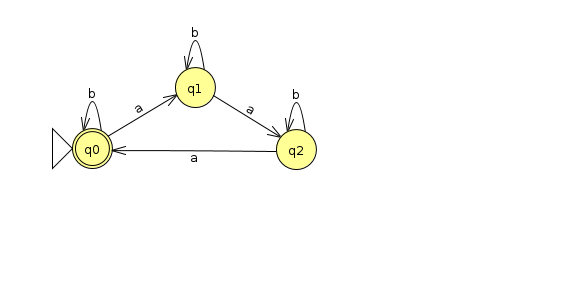
\includegraphics[width=.5\textwidth]{1_43.png}
\end{center}


Formally, Every language, $A$, represents a set of strings that are accepted. We define the DROP-OUT operation to take a string  $xyz \in A$, and remove a symbol. We are also able to represent $A$ as a regular expression that is the union of every string $xyz$ where $xyz \in A$. We also know that every string of symbols,$xyz \in A$ is a regular expression. Since we know that all $xyz \in A$ are merely strings of characters that are elements of $\Sigma$, and we can safely remove one symbol from any string (besides the empty string which has no symbols to remove but is still a valid regular language) and still have that string, $xy$, be a regular language. Since this is what the DROP-OUT operator does, we know that even when DROP-OUT is called on $A$, $A$ can still be represented as the union of a number of regular languages, thus making $A$ a regular language. Since DROP-OUT($A$), where $A$ is a regular language, yields a regular language as its output, we know that regular languages are closed under the DROP-OUT operation.

\end{document}
